\chapter{绪\quad 论}\label{ch:introduction}

\section{研究背景与问题提出}\label{sec:background}

\subsection{传染病监测的世纪演进：从宏观仓室到微观统计推断}
自二十世纪初近代数理流行病学创立以来，定量刻画传染病传播动态、评估防控干预成效一直是应用数学、统计学与公共卫生交叉领域的核心前沿。1927 年，Kermack 与 McKendrick 提出了划时代的确定性仓室易感--感染--移出（SIR）常微分方程模型 \citep{kermack1927contribution}，首次奠定了通过微分方程动力系统定性理论研究传染病临界暴发阈值的理论根基。在过去的近一个世纪中，以 Anderson 与 May \citep{anderson1991infectious}、Hethcote \citep{hethcote2000mathematics} 以及马知恩先生学派 \citep{ma2001stability,ma2004epidemic} 为代表的学者们，将常微分方程稳定性理论、下一代矩阵法 \citep{diekmann1990definition,diekmann2000mathematical} 与分岔分析深入引入传染病动力学，确立了基本再生数 $\mathcal{R}_0$ 作为无病平衡点局部与全局渐近稳定性的核心判据。

然而，经典确定性微分方程仓室模型本质上依赖于“大数定律完全成立”的流体极限假定（Fluid Limit Theorem）\citep{kurtz1970solutions,kurtz1971limit}，即假设易感人群与感染人群规模无限大、个体接触完全均匀混合、系统演化完全遵循确定性均值轨道。进入二十一世纪，随着全球化人口流动加剧、新型呼吸道病原体（如 SARS、高致病性禽流感、H1N1 新型流感及 COVID-19）频繁爆发，真实疫情传播展现出高度复杂的随机性特征。一方面，真实世界中的传染病暴发始于少数感染个体的微观随机链式反应，必须借助随机生灭过程与 Galton--Watson 分支过程进行建模 \citep{harris1963theory,jagers1975branching,britton2010stochastic}；另一方面，流行病学决策者往往无法直接观测到全社会底层的全部感染状态，只能通过哨点医院网络记录到带有严重滞后与漏报的病例计数时序序列。

在此背景下，传染病监测的推断范式经历了从“基于大样本长时程拟合静态参数”向“基于实时观测病例流估计时变瞬时再生数 $R_t$”的深刻转变。时变再生数 $R_t$ 定义为在 $t$ 时刻特定的防控干预、气象环境与人群行为条件下，平均一个感染者引发的二次感染人数。由于 $R_t = 1$ 精确对应了动力系统在相空间中的稳定临界分界线，实时监测 $R_t$ 是否越过 1 成为指导学校停课、医疗资源调度与口罩令实施的关键决策指针。

\subsection{公共卫生应急决策中的“规模崇拜”困境与现实悖论}
伴随现代生物检测技术通量的激增与数字化疫情直报网络的普及，公共卫生监测实践中普遍滋生了一种强烈的经验预设，即所谓的**“监测规模崇拜”**（Surveillance Scale Worship）。这一直觉认为：
\begin{quote}
\textit{“捕获的数据越多越好，样本量越大推断越准。只要疾控机构不断增加检测哨点、扩大医院上报覆盖面、增加报告确诊人数（即增大病例样本规模 $m$），统计推断与前瞻预测的不确定性就能被无界压缩。”}
\end{quote}
这一直觉在纯粹的数理统计抽样理论中似乎不言自明——大数定律与中心极限定理指出，独立同分布样本均值的估计方差随样本量按 $O(1/m)$ 速率严格递减，因此投入更多资源捕获更多病例，理应获得更高的预测精度。

然而，在多次全球性重大传染病暴发的应对实务中，世界卫生组织（WHO）及各国疾控中心频繁陷入极其尴尬的现实困境：
\begin{enumerate}[label=(\arabic*)]
    \item **高峰期预测精度平台瓶颈**：在疫情高发暴发期，医疗监测系统每周能捕获成千上万例确诊住院病例，但前瞻预测模型的相对误差往往依然居高不下；
    \item **边际扩网收益锐减**：卫生部门投入巨额财政资金成倍扩建检测网络后，对未来趋势判断的改善却极其微弱，迅速陷入明显的平台钝化期；
    \item **资源错配困境**：在疫情低发期或早期，由于病例稀疏，系统饱受抽样噪声干扰而频繁产生虚警或漏报；而在高发期，巨额采样资源堆积在已被证实处于饱和状态的大型医院，造成基层流调资源的严重浪费。
\end{enumerate}

面对这一现实矛盾，流行病学界以往多笼统地归咎于“医院瞒报漏报”、“公众就医行为改变”或“具体预测模型结构设定不当”。但这些定性解释始终未能回答一个根本性的数学与统计学科学设问：
\begin{center}
\textbf{在资源受限情境下，无限扩大病例报告规模的边际方差收益何时递减？\\微观抽样误差与宏观环境噪声究竟如何抗衡？\\是否存在一个内生决定且可严格解析计算的特征规模临界平衡点？}
\end{center}

\section{国内外研究现状与文献综述}\label{sec:literature}

为了系统厘清上述科学设问的学术渊源，本节系统梳理时变再生数估计、超传播离散建模、信息论极限及运筹抽样设计的既有研究脉络，并剖析既有理论的关键缺口。

\subsection{时变再生数估计方法的演进历程}
在实时再生数估计领域，早期的经典方法依赖于回顾性代际追踪。Wallinga 与 Teunis \citep{wallinga2004different} 提出了基于病例对（Pairwise）相对发病时间间隔概率的拟似然估计法（WT 方法）。然而，WT 方法本质上估计的是“病例队列再生数”（Case Reproduction Number），即一个特定发病日期的感染者在其整个病程中引发的总后续感染数，这导致其在疫情当周无法实时结算，必须等待一个完整潜伏传播周期后才能完成回顾性后验修正，存在长达数周的结构性时滞 \citep{cauchemez2006real,fraser2007estimating}。

为了消除这一回顾性时滞，Fraser \citep{fraser2007estimating} 提出了基于更新方程（Renewal Equation）的瞬时再生数理论框架。在假定感染代际时间（Generation Time）分布已知的前提下，当期新发感染数可表示为历史感染压力的加权卷积：
\begin{equation}
I_t = R_t \sum_{s=1}^t I_{t-s} w_s,
\end{equation}
其中 $w_s$ 为代际间隔概率密度。随后，Cori 等人 \citep{cori2013new} 在《American Journal of Epidemiology》上发表了标志性的 EpiEstim 框架。EpiEstim 假设在滑动的局部时间窗口 $\tau$ 内传播强度恒定，假定观测病例在给定历史卷积压力下服从泊松分布，并利用共轭 Gamma 先验导出了后验分布的解析闭式解。Thompson 等人 \citep{thompson2019improved} 进一步将该框架推广至考虑输入病例与本土病例分化的场景；Gostic 等人 \citep{gostic2020practical} 则系统评估了就医填报时滞反卷积平滑对 EpiEstim 稳定性的影响。

然而，EpiEstim 及其衍生方法的核心假设均建立在**“条件独立泊松分布”**之上。在数理统计上，泊松分布强制方差等于均值，这一假定严重忽略了真实人类传染病中普遍存在的微观超传播特征。

\subsection{微观生物学超传播与过度离散建模}
真实传染病的传播过程绝非均匀微观相遇。2005 年，Lloyd-Smith 等人 \citep{lloydsmith2005superspreading} 在《Nature》上发表了奠基性论文，通过对全球 8 种传染病的历史个体接触追踪数据进行元分析，证实人类传染病普遍遵循“20/80 法则”——即大约 20\% 的高感染力个体引发了全社会 80\% 的二次感染事件（所谓的“超级传播事件”，Superspreading Events, SSEs）。

Lloyd-Smith 等人提出用 **负二项分支过程（Negative Binomial Branching Process）** 替代经典泊松分支过程，其微观机制是个体感染力服从 Gamma 混合泊松分布：
\begin{equation}
Y_{t,j} \mid \nu_{t,j} \sim \Poisson(\nu_{t,j}), \quad \nu_{t,j} \sim \GammaDist\left(k, \frac{R_t}{k}\right),
\end{equation}
从而积分边缘化导出个体子代二元分布 $Y_{t,j} \sim \NB(k, \frac{k}{k+R_t})$，其方差结构为：
\begin{equation}
\Var(Y_{t,j}) = R_t + \frac{R_t^2}{k}.
\end{equation}
在此模型中，$k$ 被定义为**生物学生殖数过度离散参数**（Dispersion Parameter）。当 $k \to \infty$ 时，模型退化为经典泊松分布；当 $k \to 0$ 时，模型表现出极端的重尾特征。随后的 COVID-19 大流行研究中，Endo 等 \citep{endo2020estimating}、Althouse 等 \citep{althouse2020superspreading} 及 Sneppen 与 Simonsen \citep{sneppen2021overdispersion} 广泛证实新型冠状病毒的离散参数极低（$k \approx 0.1 \sim 0.3$），表现出极强的超传播倾向。

过度离散特性的引入，意味着微观传染具有极高的重尾随机涨落。如果疾控系统收集到的样本量有限，少量超级传播者的出现或缺席将引发剧烈的抽样方差，常规渐近正态近似将在小计数区间彻底失真。

\subsection{信息论极限与既有文献的关键缺口}
近年来，物理学家与应用数学家开始尝试利用信息论工具探究带噪疫情曲线的推断极限。2022 年，牛津大学的 Parag 等人 \citep{parag2022fundamental} 在《Nature Physics》上发表封面论文《Fundamental limits on inferring epidemic dynamics from noisy case count data》，利用 Fisher 信息矩阵（Fisher Information Matrix）与 Cramér--Rao 下界，系统推导了在不完全报告与观测噪声下估计再生数的信息量上限。

Parag 等人的核心结论表明：观测曲线所包含的 Fisher 信息量 $\mathcal{I}(R_t)$ 随观测病例数近似呈线性增长。这一结论在物理学界引起了广泛关注，但其推导隐含了一个关键前提——**其推断目标始终锚定在“当期特定微观环境下的瞬态参数 $R_t$”**。

这正是既有文献留下的**最致命的理论断裂与盲区**：
\begin{enumerate}[label=(\alph*)]
    \item **推断目标的严重混淆**：
    实际公共卫生决策者需要的往往不是某一周受微观偶然扰动影响的单期瞬态抖动值 $R_t$，而是能够反映潜在流行趋势、消除单周气象或节假日偶发波动的**跨期平稳传播基准 $\bar{R}$**。既有文献从未区分这两个目标在方差标度律上的本质分化。
    \item **忽视不可约宏观环境噪声**：
    在宏观动力学系统中，除了个体抽样的人口统计随机性（Demographic Stochasticity）外，全社会所有感染者不可避免地共同暴露于宏观气象变迁、社会流动潮汐与政策突变等**不可约环境随机性（Environmental Stochasticity）**之下。当估计跨期基准时，单期样本无论扩大到多大，本质上都只能捕获该宏观环境在该期的一个实现值！
    \item **缺乏运筹维度的经济学对偶**：
    既有流行病学研究多停留在“被动给定样本下评估误差”，鲜有将统计推断方差分解与实际监测网络的运作预算、时间抽样期数与单期规模进行联合运筹优化。
\end{enumerate}

表~\ref{tab:literature_comparison} 系统总结了本文与既有标志性文献在建模维度与推断性质上的本质对比。

\begin{table}[htbp]
\centering
\small
\caption{本文与既有核心文献在模型机制与推断理论维度的系统对比}
\label{tab:literature_comparison}
\begin{tabularx}{\textwidth}{lXXXX}
\toprule
\textbf{比较维度} & \textbf{经典仓室 ODE (Kermack)} & \textbf{EpiEstim 框架 (Cori 2013)} & \textbf{信息论界限 (Parag 2022)} & \textbf{本文理论框架} \\
\midrule
\textbf{微观生成机制} & 宏观确定性连续流体 & 条件独立泊松分布 & 状态空间观测模型 & 负二项超传播分支过程 \\
\textbf{宏观报告环节} & 假定完全无偏报告 & 静态先验平滑假定 & 独立乘性高斯/泊松噪声 & 条件二项报告抽稀保族过程 \\
\textbf{核心推断目标} & 静态渐近参数 $\mathcal{R}_0$ & 局部滑窗时变 $R_t$ & 单期瞬态连续参数 $R_t$ & **区分瞬态 $R_t$ 与跨期基准 $\bar{R}$** \\
\textbf{环境变异考量} & 无（确定性流形） & 无（完全吸收入先验） & 视为普通可加测量噪声 & **显式建模不可约环境方差 $v_R$** \\
\textbf{规模收益结论} & 无样本规模维度 & 样本越大后验方差越小 & 信息量随病例数线性增长 & **存在内生特征平衡点 $m_\times$** \\
\textbf{运筹成本对偶} & 无 & 无 & 无 & **同构于 Cochran 两阶段抽样** \\
\textbf{真实大数据检验} & 历史唯象拟合 & 局部小样本演示 & 数值仿真为主 & **全美 1.6 万记录与外部多病种** \\
\bottomrule
\end{tabularx}
\end{table}

\section{本文研究动机与核心科学贡献}\label{sec:contribution}

\subsection{核心研究动机}
立足于上述理论断裂与现实困境，本文旨在打破“规模越大越好”的传统单一教条，建立一套贯通**“微观超传播分支过程 $\to$ 宏观二项报告抽稀 $\to$ 渐近推断方差分解 $\to$ 运筹抽样设计 $\to$ 真实大数据计量检验”**的完整理论与实证闭环体系，精准回答流行病学监测资源何时应当由“单纯扩充数量”转向“结构性协同提质”。

\subsection{主要学术贡献}
本文的核心学术创新可概括为以下四项支柱性贡献：

\begin{enumerate}[label=\textbf{\arabic*.}]
    \item **理论框架破局：确立“推断目标决定规模收益”的方差标度律分化**\\
    本文从微观概率母函数（PGF）复合律出发，严密证明了负二项分支过程在二项抽样下具有严格的分布族封闭性。在此基石上，本文证明：
    若目标为当期瞬态再生数 $R_t$（目标 A），估计量方差达到 Cramér--Rao 下界并随规模 $m$ 按 $O(1/m)$ 无界衰减；
    若目标为跨期基础传播基准 $\bar{R}$（目标 B），全方差分解严格导出了包含不可约环境方差底板 $v_R$ 的仿射损失结构：
    \begin{equation}
    \Var = v_R + \frac{A}{m},
    \end{equation}
    并内生导出了刻画人口统计随机性向环境随机性跃迁的特征规模平衡点 $m_\times \equiv A/v_R$。
    
    \item **运筹机制创新：证明监测杠杆非对称性与 Cochran 两阶段抽样对偶**\\
    在监测杠杆比较上，本文严格证明了提高报告率 $\rho \to 1$ 无法突破微观泊松与超传播方差下界，而扩大风险基数 $n \to \infty$ 方可使方差收敛至 $v_R$。
    在运筹设计上，本文证明在固定总样本人数预算 $B = T m$ 下微观抽样误差恒为常数 $A/B$；并在显式经费预算约束 $\mathcal{B} = T(c_0 + c_1 m)$ 下证明了目标方差函数的严格凸性，推导出最优单期规模闭式解 $m^* = \sqrt{\frac{c_0}{c_1} m_\times}$，在数学结构上完美同构于经典抽样调查 Cochran 两阶段最优分配模型。
    
    \item **数理与仿真深化：解析离散功效锯齿波与更新过程预测双口径机制**\\
    针对爆发早期假设检验 $H_0: R_t \le 1$，本文证明单调似然比（MLR）一阶对数差分严格为正，利用 Karlin--Rubin 定理构造了 UMP 检验，揭示了离散计数阶梯跳跃引发的功效锯齿波机制，证实检验目标存在天然饱和天花板 $m_{80\%}$。在更新过程时间序列预测中，推导了条件预测方差分解式，阐明了用历史卷积代理真实感染所必然引入的额外非负预测偏差项，彻底澄清了初始参数口径与实际实现规模口径下的参照收敛性。
    
    \item **真实大数据实证：全美六年流感住院实证反转与外部多病种跨场景验证**\\
    基于全美 CDC NHSN 覆盖 50 州及 DC 长达六年的 16,218 条真实住院面板数据（客观筛选 10,303 个活跃周），采用可行广义最小二乘法（FGLS）与 1,500 次聚类 Bootstrap 检验，证实规模反比项高度显著为正（$\hat{b} = 2.2434$，CI $[1.50, 3.02]$），经验平衡点约为 22.6 例/周。
    均值--方差正交分解惊人地揭示，达峰期看似恒定的高误差中 88.9\% 源于基准失配，扣除后规模项依然显著有用，有力推翻了“达峰期样本量失效”的传统误读；
    进一步引入 CDC FluSight 官方集成预测（达峰偏差从 88.9\% 骤降至 15.5\%）与欧洲 11 国 COVID-19 数据，证实了多模型集成对系统漂移的校准价值及仿射规律跨病种的稳健性。
\end{enumerate}

\section{论文结构安排与技术路线}\label{sec:outline}

为系统展现本文的逻辑流向与整体研究脉络，图~\ref{fig:technical_roadmap_ch1} 给出了贯通全书的“多源输入 $\to$ 微观分支机制 $\to$ 渐近推断方差理论 $\to$ 运筹优化设计 $\to$ 真实大数据实证与政策矩阵”的端到端技术路线全景架构。

\begin{figure}[htbp]
\centering
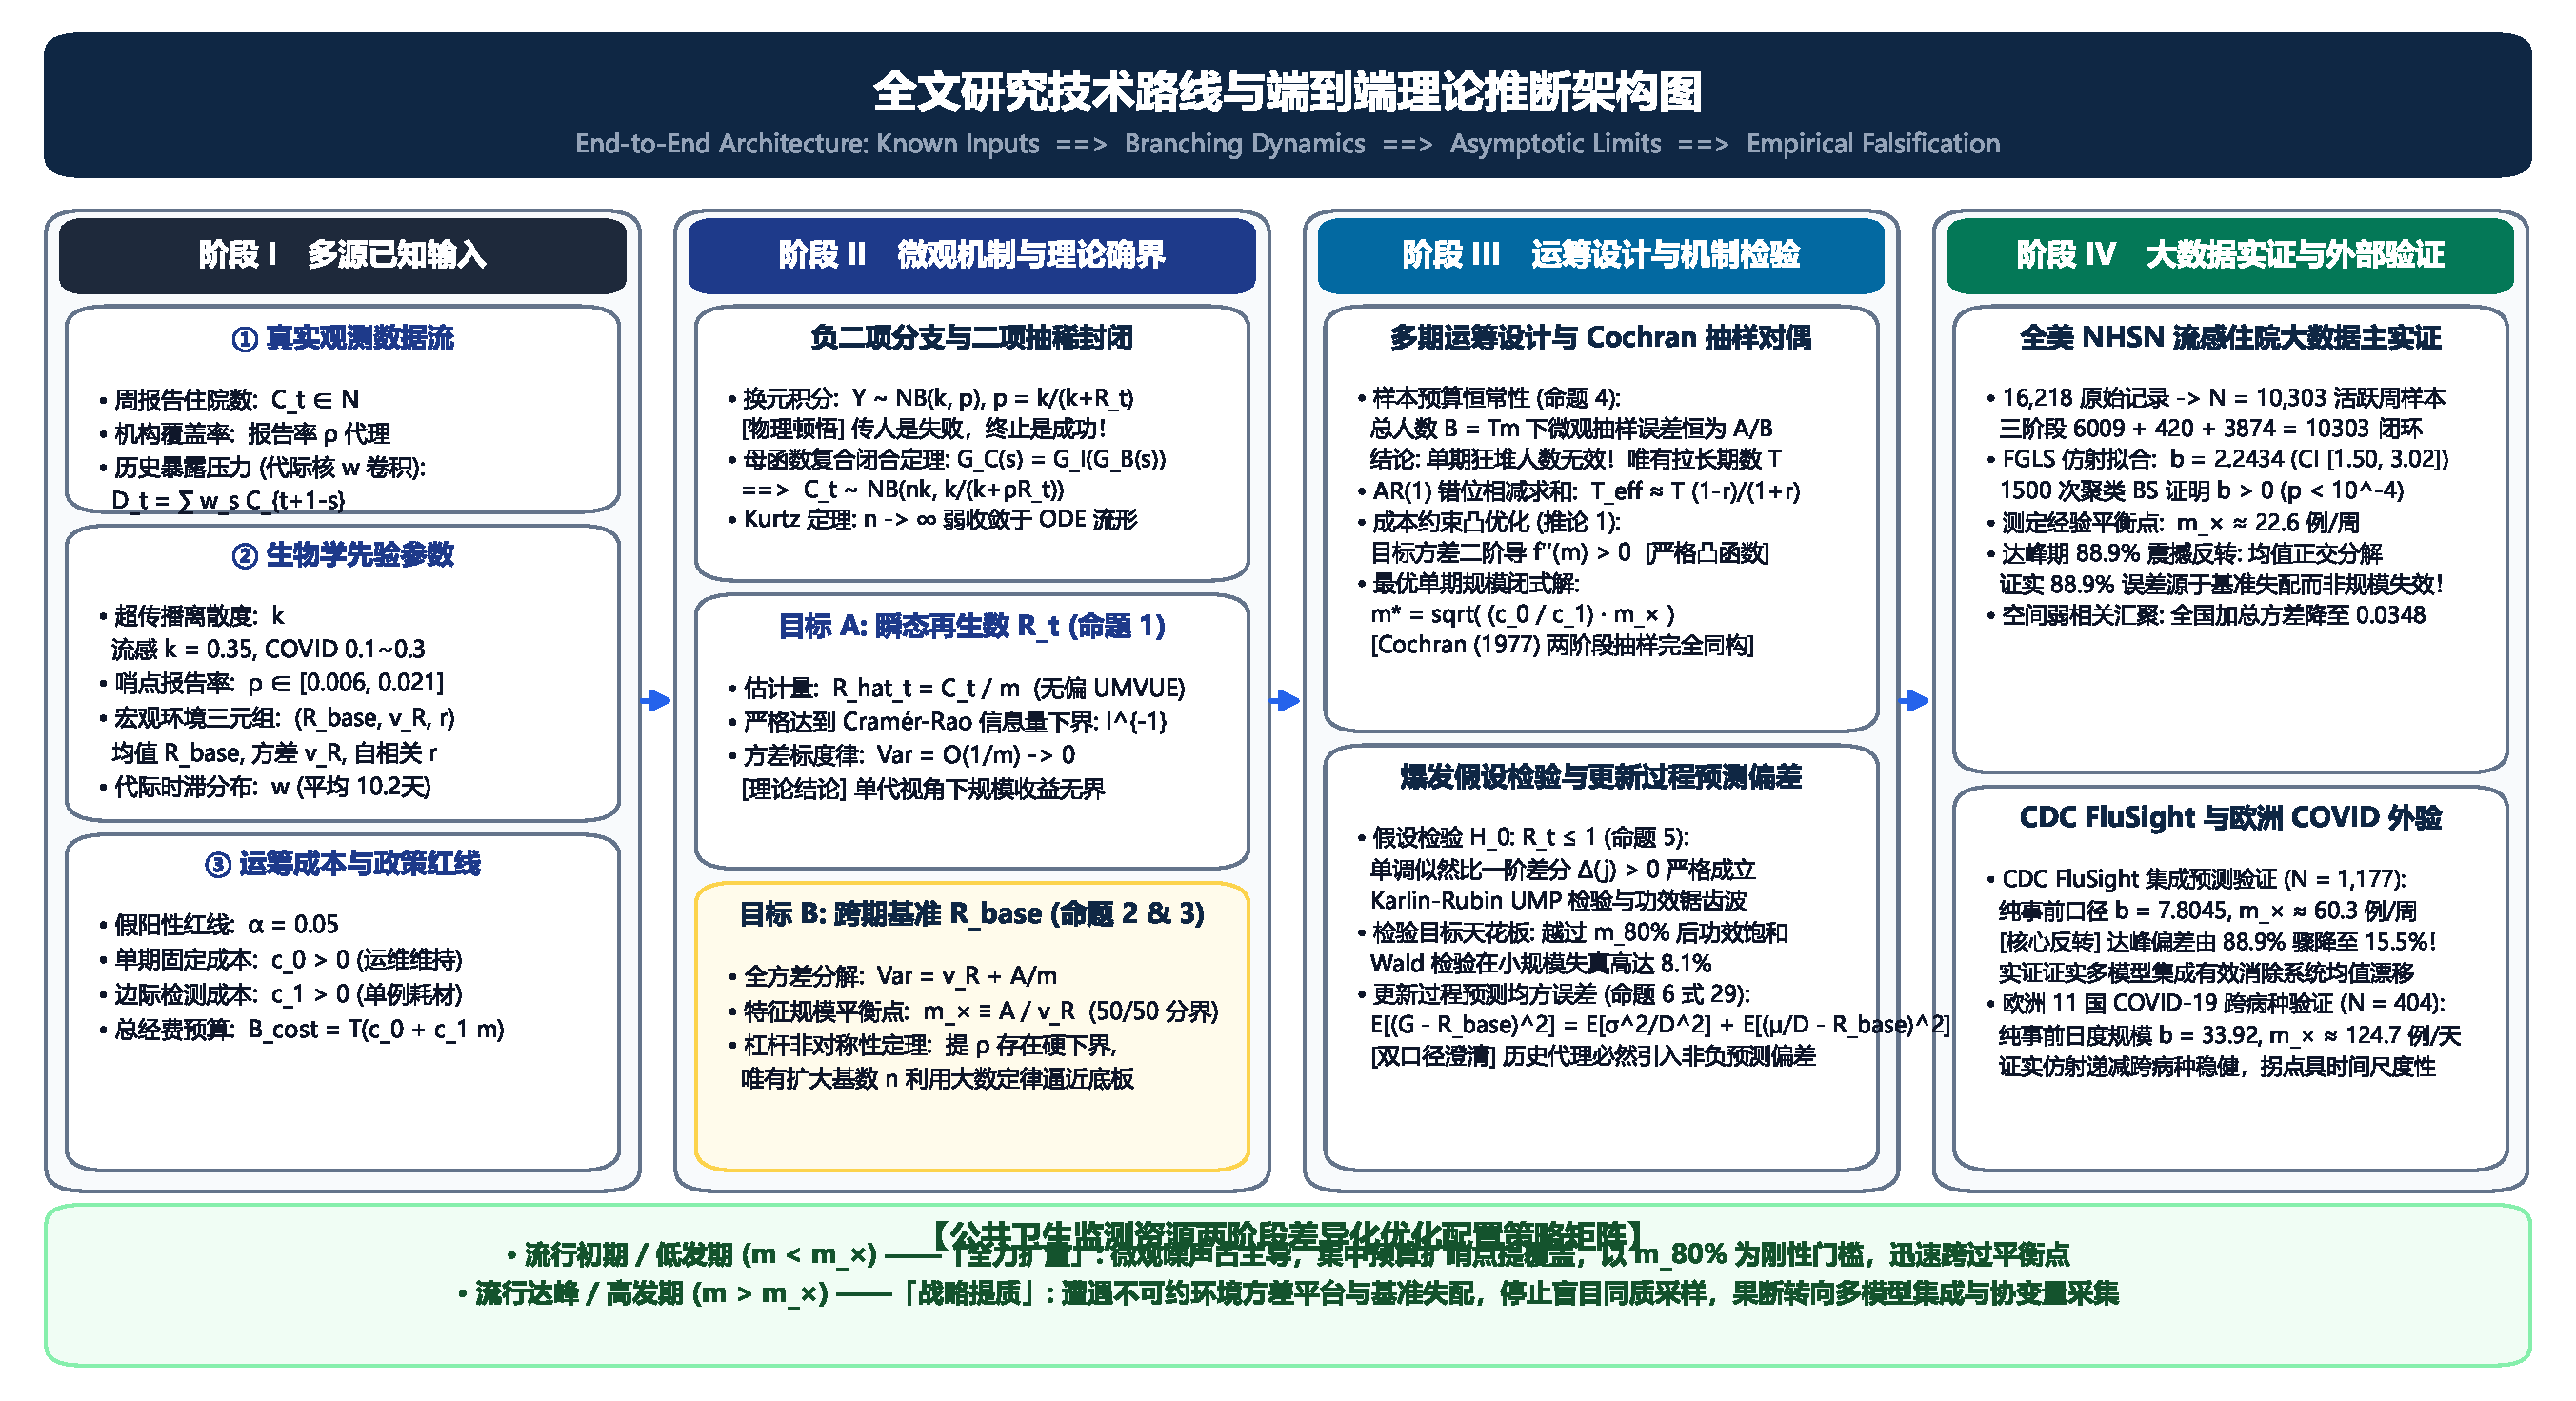
\includegraphics[width=\textwidth,height=0.38\textheight,keepaspectratio]{figures/fig0_technical_roadmap.pdf}
\caption{\textbf{全文研究技术路线与端到端理论推断全景架构图。} 展示从已知输入（真实观测数据流、生物学先验参数与运筹成本约束）到微观分支机制、渐近推断方差分解（目标 A 与目标 B 的分化）、监测运筹优化（Cochran 抽样对偶）、假设检验天花板，直至全美真实流感住院大数据计量检验与公共卫生决策矩阵的端到端逻辑闭环。}
\label{fig:technical_roadmap_ch1}
\end{figure}


本学位论文其余部分的组织架构安排如下：

\textbf{第二章：动力学建模与观测机制}。从微观生灭分支过程出发，展开个体传染力 Gamma 连续混合积分推导；深入阐释成功概率 $p = \frac{k}{k+R_t}$ 与抽稀后 $p^*$ 的统计物理顿悟；通过概率母函数复合律严格证明二项抽稀保族封闭性；并在第 2.4 节建立微观随机分支过程与宏观确定性仓室常微分方程系统的 Kurtz 流体极限动力学理论桥梁。

\textbf{第三章：渐近推断与运筹优化理论}。严格形式化定义推断目标 A 与目标 B；给出命题 1 条件似然、得分方程、双层全期望塔式法则无偏性证明与 Fisher 信息双套算法（UMVUE）；推导命题 2 跨期全方差仿射分解；证明命题 3 监测杠杆理论非对称性；给出命题 4 多期时间抽样预算恒常性与 AR(1) 错位相减求和闭式解；证明推论 1 成本优化严格凸性与 Cochran 抽样对偶。

\textbf{第四章：蒙特卡洛仿真与机制检验}。介绍 Python 蒙特卡洛随机模拟实验规格；检验命题 5 超临界增长精确检验、MLR 一阶差分、离散功效锯齿波与 Wald 正态失真；验证命题 6 更新过程单步预测两步全方差分解与式 (29) 预测偏差项；系统澄清图 1、图 2、图 3 的双口径参照关系。

\textbf{第五章：全美流感住院大数据实证分析}。详细梳理全美 CDC NHSN 监测系统背景、16,218 条原始记录筛选至 10,303 样本的客观漏斗与三大制度期算术闭环；针对重尾异方差构建 FGLS 计量拟合；汇报流行初期核心估计结果；展开达峰期 88.9\% 偏差正交分解反转；评估 2024 年自愿填报政策冲击与全国 51 辖区空间汇聚对偶收益。

\textbf{第六章：跨模型与跨病种外部扩展验证}。阐述外部验证的设计原则；汇报 CDC FluSight 官方多模型前瞻集成预测实证结果，展示多模型集成将达峰偏差压缩至 15.5\% 的去偏机制；汇报欧洲 11 国早期 COVID-19 纯事前日度发病实证结果，论证仿射递减项的跨病种普适性与经验平衡点的尺度敏感性。

\textbf{第七章：监测资源优化策略与研究展望}。构建国家公共卫生监测体系在不同流行阶段的“差异化两阶段资源配置策略矩阵”；深入剖析当前研究将平衡点作为拟合量而非测量量的方法学局限；提出基于前瞻性主动社区追踪队列的双轨解耦识别设计；对全文核心结论进行总结。

\textbf{附录 A} 提供论文所有命题与推论的保姆级中间推导展开细节。
